\documentclass[a4paper, 11pt]{article}
\usepackage{comment} % enables the use of multi-line comments (\ifx \fi)
\usepackage{lipsum} %This package just generates Lorem Ipsum filler text.
\usepackage{fullpage} % changes the margin
\usepackage[utf8]{inputenc}
\usepackage{color}
\usepackage[usenames,dvipsnames]{xcolor}
\usepackage{hyperref} 	%% Use to fix Figure or Table: ex: \begin{table}[H]
\hypersetup{
	%pagebackref=true,
	pdfcreator={LaTeX with abnTeX2},
	pdfkeywords={abnt}{latex}{abntex}{USPSC}{trabalho acadêmico},
	colorlinks=true,       		% false: boxed links; true: colored links
	linkcolor=blue,          	% color of internal links
	citecolor=blue,        		% color of links to bibliography
	filecolor=magenta,      		% color of file links
	urlcolor=blue,
	allbordercolors=black,
	bookmarksdepth=4
}
\usepackage[portuguese]{babel}
\usepackage{graphicx}

\begin{document}
\noindent
\normalsize
 \textbf{Relatório 3, bolsa TT5, processo 2017/14778-4}\\
Processo vinculado: \textbf{2017/05838-3} \\
Coordenadora: \textbf{Dra. Maria Cristina Ferreira de Oliveira} \\
Bolsista: \textbf{Dr. Renato Fabbri}

\section{Informação sobre o nível e período de usufruto da Bolsa}
A bolsa é TT5 (Treinamento Técnico nível 5), vigente de 01/Set/2017 até 30/Jun/2019.
O período referente a este relatório é de 31/Jul/2018 até 30/Ago/2019,
de acordo com a prorrogacao concedida pela FAPESP.
Eu, o bolsista, continuo, de 30/Ago/2019, ate hoje, 17/Dez/2019, em atividade eventual, 
por escolha própria, principalmente mantendo comunicacao com pesquisadores e
mantendo as ferramentas disponibilizadas online.
Também, por exemplo, para a entrega deste relatorio na data correta.

\section{Atividades realizadas e em andamento}\label{desc}
As principais contribuicoes estao descritas nas proximas secoes.
Visei aplicar meus conhecimentos e proficiências nas atividades previstas no projeto desta bolsa TT5
e no projeto de pesquisa associado.
Devido ao período curto assiciado à renovacao, e ao formato curto requisitado
para este relatório, este documento estende o relatório 2
desta mesma bolsa, evitado repetir as informações.

\subsection{Visualização interativa de redes bipartidas assistida por estratégias multinível}\label{sml}
Em colaboração com os pesquisadores Alan Valejo, Alneu Andrade, e Cristina Oliveira,
implementei uma forma de navegação das redes em representação multinível
utilizando arestas híbridas. A navegação descrita no relatório 2 utiliza retângulos translúcidos
para manter (sub-)vértices agrupados em seus super-vértices, representa os (sub-)vértices nos retângulos.
Nesta nova navegação, reiterada pelo Alan como intuitiva e talvez ideal como modelo de referência,
quando um super-vértice é expandido/aberto, os sub-vértices sao postos no canvas individualmente, sem
o agrupamento pelo super-vértice original, e arestas envolvendo estes vértices são:
1) com vizinho, se vizinho representado;
2) com pai do vizinho, se pai do vizinho representado;
3) com filhos do vizinho, se filhos do vizinho representados.

As arestas implicadas por 2) e 3) são arestas híbridas.
Este modelo implica na necessidade de ajustes no layout quando
os super-vertices sao expandidos ou colapsados.
Portanto, esta implementacao envolve tambem layout em tempo real,
e novos algoritmos de layout (teoricamente) os mais leves possivel.

Planejamos dois incrementos para as interfaces desenvolvidas nesta linha de atuação:
adicionar novamente as widgets e funcionalidades relacionadas aos histogramas
de grau e coeficiente de clusterizacao.
Integrar o BNOC~\cite{bnoc}, ferramenta para síntese de redes bipartidas.
Assim, ate a entrega da versao final deste relatorio (30/Jan/2019),
planejamos ter uma interface de visualizacao consistente para o estudo de estrategias
multiniveis em redes bipartidas, e incrementos no artigo rejeitado (descrito no relatório anterior)
para ressubmissão.

Para melhorar a qualidade do software, sem prioridade no momento,
concebemos algumas tarefas principais.
Sao ``issues'' para serem vinculadas ao repositorio Git principal:
refatorar e limpar o codigo para separar as aplicacoes;
loop assíncrono para calculo de posicoes dos vertices,
atualizando quantos loops conseguiu realizar, para auxiliar o usuário a escolher um algoritmo de layout de rede;
\emph{particle system} para vértices e arestas (já testei em novos experimentos, permite a visualização de redes muito maiores. Uso da GPU para cálculo vetorial (importante para obter layouts de redes).  Aplicacao mais voltada para ``visual analytics'' considerando os metadados. Fazer um script Bash para colocar no ``cron'' e subir as interfaces sempre que for dado reboot no servidor.

    A nova interface está acessível publicamente em \url{http://rfabbri.vicg.icmc.usp.br:3000/multilevel2/topdown2}, e o vídeo expositivo em \url{https://youtu.be/VdAVE4AHfi8}.
    A Figura~\ref{ml} exemplifica a interface em uso.

\begin{figure}[h!]
\centering
  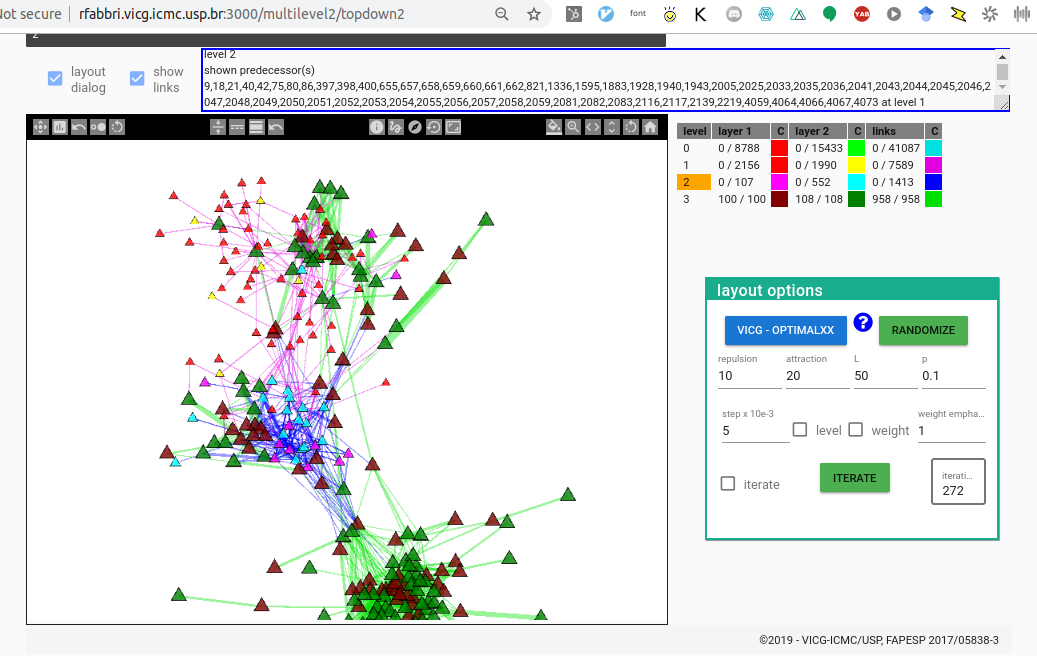
\includegraphics[width=0.8\linewidth]{hybrid}
\caption{%
  Para além do descrito no relatório anterior, note os vértices de 3 níveis diferentes, relacionados por arestas
  híbridas, sem a utilização de caixas para super-vértices expandidos.
  Note também o componente para cálculo das posições dos vértices (i.e. do 'layout de rede') em tempo real.
}\label{ml}
\end{figure}

\subsection{Visualização interativa de redes utilizando comunicabilidade}\label{scom}
Na continuidade da colaboração com Ernesto Estrada, pesquisador notório em Redes Complexas, autor de livros e de diversas publicações relevantes para a área~\cite{ern1,ern2,ern3,ern4},
ele apresentou a interface já na ``Latin American Conference on Complex Networks'' (5-9/Ago/2019):
\url{http://rfabbri.vicg.icmc.usp.br:3000/communicability}.
Esta interface passou por diversas versões, recebeu novos algoritmos de clusterizacao e de reducao de dimensionaldiade, melhoras no uso das medidas de comunicabilidade, etc. A Figura~\ref{com} ilustra a forma atual da interface.
Iniciamos a escrita do artigo a ser submetido sobre o software desenvolvido e dua utilidade.

\begin{figure}[h!]
\centering
  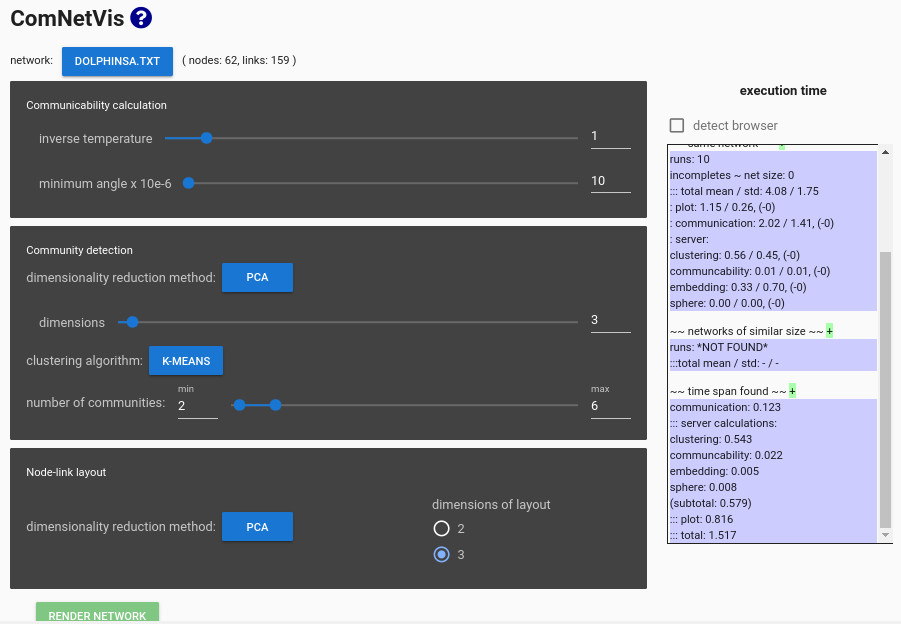
\includegraphics[width=0.8\linewidth]{com}
\caption{%
  Solução final encontrada em conjunto com o pesquisador Estrada.
  Foi fixado o uso dos ângulos de comunicabilidades, e descartado o uso das distâncias.
  Há uma redução de dimensionalidade para a detecção de comunidades,
  outra para a obtenção das posições no plano ou espaço 3D.
  Há diversos métodos de clusterização.
  Fez-se também necessária a manuteção dos tempos associados às execuções,
  pois alguns dos métodos são custosos quando há muitos vértices e/ou arestas.
}\label{com}
\end{figure}


\subsection{Interface para visualização e análise de redes longitudinais}\label{sevo}
Iniciamos a consideracao do artigo rejeitado para ressubmissao.
As revisões obtidas na rejeição pareceram positivas quanto às contribuições potencialmente
novas do trabalho. Há, porém, a necessidade de melhor contextualizar e disponibilizar a ferramenta
com facilidades para o uso por uma pessoa não interna à pesquisa.

\subsection{Interface para visualização de redes enriquecidas com texto}
A interface mínima já implementada (\url{https://youtu.be/MH1D8S75d7E}),
continua em consideração e amadurecimento para descrição a aprodundamento
do modelo mínimo de visualização com técnicas de redes complexas, mineração
de texto, e distâcias estatísticas.

\subsection{Visualização para auxílio à análise de paisagens sonoras}\label{pa}
Desenvolvemos uma nova interface de análise de paisagens sonoras com base no
artigo~\cite{eld}.  
Nesta nova versao, o usuario pode adicionar arquivos de áudio ou escolher algum dos disponíveis.
Pode também escolher o número de componentes para a decomposição do som original,
e o código está preparado para adicionar customizações.
As possibilidades de parametrização do SIPLC2D são muitas, portanto estamos avaliando quais
parametrizações devem ser disponibilizadas na interface.
Além disso, dado que não conseguimos (ainda) decompor o som original nas componentes de um
trecho menor, por enquanto decidimos permitir a análise de um trecho pequeno para escolha da
parametrização a ser aplicada em todo o áudio, pois o método é computacionalmente custoso.
A Figura~\cite{ps} exemplifica a interface em operacao.
Esta nova interface está disponível em: \url{http://rfabbri.vicg.icmc.usp.br:3000/soundscape/min},
enquanto a interface inicial foi realocada para: \url{http://rfabbri.vicg.icmc.usp.br:3000/soundscape}.

A Figura~\ref{ss} ilustra a forma atual da interface.

\begin{figure}[h!]
\centering
  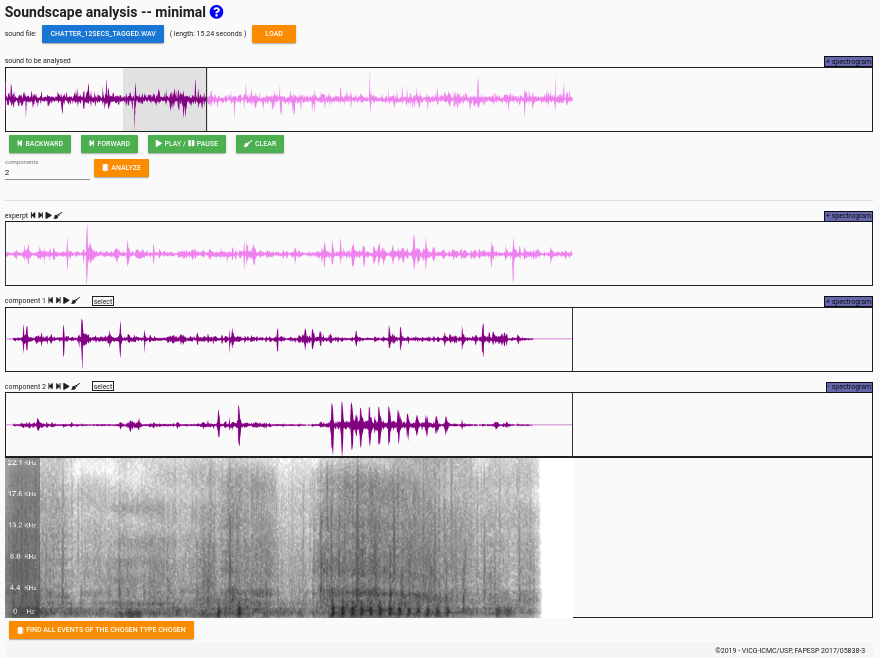
\includegraphics[width=0.8\linewidth]{ss}
\caption{%
  A versão expandida da interface mínima para utilização de SIPLC2D na separação de fontes sonoras.
  Nesta versão, o usuári pode subir novos arquivos de áudio, escolher o áudio para análise,
  escolher o trecho para análise, o número de componentes, e ouvir individualmente cada componente
  ou o trecho escolhido para análise.
  O usuário também pode observar o histograma de qualquer componente, e pode fazer uso de algumas
  funcionalidades para a seleção e audição de trechos de áudio.
}\label{ss}
\end{figure}

\subsection{Disponibilização de dados ligados de redes sociais}
Para dar suporte à pesquisa realizada no VICG, entrei em contato com o
Data.World (apresentado para mim pela profa. Cristina, coordenadora do projeto)
e estabeleci uma colaboração.
Pudemos então disponibilizar publicamente, em RDF, dados das seguintes redes sociais:
Facebook, Twitter, Email, IRC, Participa.br, Cidade Democrática, AA.
Ao todo, estes dados formam uma rede com centenas de milhares (talvez até alguns milhões)
de participantes, relacionados em geral por amizades, interações, ou critérios de semelhança.
Os dados estão disponíveis em:
\url{https://data.world/rfabbri/linked-open-social-data}.
Foi possível também disponibilizar uma biblioteca oficial e simples para o acesso a estes dados,
sem a utilização direta da API do Data.World ou a necessidade de quaisquer credenciais:
\url{https://pypi.org/project/losd/}.
Um artigo com uma descrição suscinta destes dados está disponível em:
\url{https://github.com/ttm/linkedOpenSocialDatabase/raw/master/mdpi/template.pdf},
com arquivo suplementar em:
\url{https://github.com/ttm/linkedOpenSocialDatabase/raw/master/supplementaryDocument.pdf}.


\subsection{Experimentos de visualização para escalar iniciativas sociais}
Em continuidade aos trabalhos reportados em~\cite{tese,virus,sfvideo},
para testar a aplicabilidade das estratégias multiníveis na ``coleta e difusão de informação e bens'',
ou na ``propagação de tratos sociais'', iniciei a escrita de software para alcançar interfaces
que permitam ao usuário iniciar processos de interação sociais em cadeia, i.e. que envolvem
a propagação de alguma informação (e.g. uma proposta).
Estes testes iniciais foram aproveitados para testar sistemas de partículas (recurso WebGL),
medições de duração (para otimização) e projeções planares.
Os códigos desenvolvidos estão todos em JavaScript e são executados no cliente,
com carga mínima para o servidor,
incluindo acesso aos dados ligados, derivação de redes, e obtenção de sequência de redes
em estratégia multinível.
O framework utilizado difere dos anteriores, com foco em Meteor.js,
nas biblitecas Pixi.js (para mapeamentos visuais de dados e elementos visuais interativos),
Tone.js (para mapeamentos sonoros dos dados),
e em requisições HTTP com \emph{queries} SparQL para acesso dos dados da LOSD.
A Figura~\ref{exp} ilustra minimamente as interfaces desenvolvidas.

\subsection{Parcerias internacionais}
A primeira autora do artigo~\ref{eld}, Alice Eldridge,
manteve contato comigo depois que escrevi para ela sobre
os métodos, para as interfaces mencionadas na Seção~\ref{}.
Em email recente, ela manifestou interesse em
estabelecer uma colaboração academica com nossa pesquisa, e que ``está já
vasculhando as oportunidades para obter verba e formalização da parceria,
no novo contexto de Brexit'' (ela trabalha na Universidade de Sussex).
O Ernesto Estrada manifestou interesse na continuidade do desenvolvimento
das interfaces de visualização de dados para o desenvolvimento e disponibilização
de novas técnicas.
Após o período de prorrogação da bolsa, estabeleci colaboração
com empresas, em especial com a BairesDev (Argentina, Vale do Silício/EUA) e
AdRoll/NextRoll/RollWorks (Vale do Silício/EUA). 
Encaminharei estas colaborações para confluir com a continuidade dos
trabalhos realizados neste projeto, e para contato entre os pesquisadores
mais importantes para a minha atuação, a saber com a coordenadora Profa. Cristina,
e com o Dr. Alan Valejo.


\section{Avaliação do impacto das atividades do bolsista sobre o andamento do projeto}
Colaborei no desenvolvimento de métodos, programação de interfaces,
que constarão em artigos submetidos.
Acredito ter auxiliado no andamento do projeto, em conformidade com a bolsa TT5.

\section{Apreciação do desempenho do bolsista (escrita pela coordenadora)}
% para Cristina escrever
O bolsista tem grande conhecimento em métodos na área de redes complexas e em programação. Assim, tem contribuído significativamente no desenvolvimento de ferramentas que mostram-se fundamentais como provas-de-conceito de diversas técnicas investigadas no âmbito do projeto. Ele tem interagido mais intensamente com os pesquisadores que atuam na frente de pesquisa em métodos multinível em redes complexas, com potencial para interagir também com pesquisadores que atuam na frente de pesquisa em paisagens acústicas. Acredito também que o projeto apresentou a ele uma nova gama de conhecimentos em visualização de dados, abrindo novas perspectivas para a sua atuação futura como pesquisador. Minha avaliação é que o bolsista está contribuindo de maneira relevante para ampliar os resultados gerados no âmbito do projeto de pesquisa.
\bibliographystyle{unsrt}
\bibliography{pbib}

\end{document}
